\documentclass{article}


% if you need to pass options to natbib, use, e.g.:
%     \PassOptionsToPackage{numbers, compress}{natbib}
% before loading neurips_2022


% ready for submission
\usepackage[final]{neurips_2022}


% to compile a preprint version, e.g., for submission to arXiv, add add the
% [preprint] option:
%     \usepackage[preprint]{neurips_2022}


% to compile a camera-ready version, add the [final] option, e.g.:
%     \usepackage[final]{neurips_2022}


% to avoid loading the natbib package, add option nonatbib:
%    \usepackage[nonatbib]{neurips_2022}


\usepackage[utf8]{inputenc} % allow utf-8 input
\usepackage[T1]{fontenc}    % use 8-bit T1 fonts
\usepackage{hyperref}       % hyperlinks
\usepackage{url}            % simple URL typesetting
\usepackage{booktabs}       % professional-quality tables
\usepackage{amsfonts}       % blackboard math symbols
\usepackage{nicefrac}       % compact symbols for 1/2, etc.
\usepackage{microtype}      % microtypography
\usepackage{xcolor}         % colors
\usepackage{amssymb}
\usepackage{float}
\usepackage{graphicx} 


\title{CS 152 Project: Checkpoint 1}

% The \author macro works with any number of authors. There are two commands
% used to separate the names and addresses of multiple authors: \And and \AND.
%
% Using \And between authors leaves it to LaTeX to determine where to break the
% lines. Using \AND forces a line break at that point. So, if LaTeX puts 3 of 4
% authors names on the first line, and the last on the second line, try using
% \AND instead of \And before the third author name.

\author{Nathaniel Davis \\
    Tufts University \\ \And 
    Kamil Krukowski \\
    Tufts University \\
    \And Yan Zhou Chen \\
    Tufts University}

% \author{%
%   David S. Hippocampus\thanks{Use footnote for providing further information
%     about author (webpage, alternative address)---\emph{not} for acknowledging
%     funding agencies.} \\
%   Department of Computer Science\\
%   Cranberry-Lemon University\\
%   Pittsburgh, PA 15213 \\
%   \texttt{hippo@cs.cranberry-lemon.edu} \\
%   % examples of more authors
%   % \And
%   % Coauthor \\
%   % Affiliation \\
%   % Address \\
%   % \texttt{email} \\
%   % \AND
%   % Coauthor \\
%   % Affiliation \\
%   % Address \\
%   % \texttt{email} \\
%   % \And
%   % Coauthor \\
%   % Affiliation \\
%   % Address \\
%   % \texttt{email} \\
%   % \And
%   % Coauthor \\
%   % Affiliation \\
%   % Address \\
%   % \texttt{email} \\
% }


\begin{document}

\maketitle

\begin{abstract}
  \textbf{Purpose:} In this project we predict the mass spectra of molecules from their molecular fingerprints, a task which, due to the sparseness of spectrum data, we approximate by predicting which discretized spectrum “bin” contains the highest-intensity peak. This task is useful as metabolite annotation via mass spectrometry requires reference spectra for comparison; however, we lack reference spectra for millions of recorded molecules, so in-silico spectra generation helps fill these gaps. \textbf{Hypothesis:} We use feedforward neural networks with SoftMax output to generate probabilities that a given bin contains the highest peak, and to approximate the posterior of a network’s weights, we use Bayes-by-Backprop (BBB) with a multivariate Gaussian posterior approximation with three different variance assumptions: uniform variance with no covariance, independent variances with no covariance, and per-layer independent variances with covariance. For each approach, we measure average SoftMax rank of the correct bin, top-k accuracy, and calibration of bin probabilities, as well as a runtime analysis involving time to model convergence. \textbf{Evaluation Plan:} We use liquid chromatography tandem mass spectra (LC-MS/MS) data from the MassBank of North America (MoNA), a large (145k spectra) public dataset, to evaluate our models by the metrics mentioned above.
\end{abstract}


\section{Changelog}
\begin{itemize}
    \item Instead of treating the problem as a vector regression task, we instead attempt to predict which discretized spectrum bin contains the highest-intensity peak. Most spectrum bins contain values at or near zero, so most of any error/closeness metric is generated by whichever bin(s) contain(s) the highest peak(s). Therefore, if we can predict the bin with the highest peak with decent accuracy, we are well on our way to satisfying most objective metrics for the original vector regression task.
    \item To evaluate the probabilistic predictions of our models, we measure prediction calibration instead of out-of-distribution detection. The former gives us a more precise, intuitive sense of the Bayesian capabilities of our models and also does not require crisply split in-distribution and out-of-distribution sets. Molecular fingerprints are very inflexible representations based on in-distribution data and therefore completely 'drop' out-of-distribution information.

    \item We listed a host of models we intended to test in our Project Pitch, but we have now limited our approach to BBB, a more realistic problem scope given our timeline. We have also decided to implement a vanilla, non-Bayesian neural net to provide baseline estimates of non-Bayesian performance metrics.
\end{itemize}

\section{Challenges}
\begin{itemize}
    \item Given the size of our inputs/outputs, implementing BBB with per-layer full covariance matrices may prove computationally intractable.
    \item The SoftMax framing of the problem, coupled with the fact that molecular fingerprints ignore all spatial information, may not produce results of reasonable quality. 
\end{itemize}

\section{Timeline}
By Monday, 11/14
\begin{itemize}
    \item Implement vanilla neural network and decide hyperparameters - Yan
    \item Decide and implement validation strategy - Kamil
    \item Review academic references and code for focus method and baseline - Nate
\end{itemize}
By Mon 11/21
\begin{itemize}
    \item Implement and evaluate uniform variance BBB model - Yan \& Nate
    \item Implement and evaluate BBB variants - Kamil
    \item Compare model performance and begin checkpoint write up - everyone
\end{itemize}

\section{Goals}
In-silico mass spectra are frequently used as references to help annotate experimentally produced spectra, yet the uncertainty of spectra predictions is rarely reported. We aim to approximate a molecule’s mass spectrum by predicting the bin location of its highest-intensity peak given its fingerprint while reporting the uncertainty of the model. Having uncertainty estimates should aid in the process of matching experimentally produced and synthetic spectra. We model this as a multiclass classification task with a training set of observations: $\{x_{1:N}, y_{1:N}\}$ where each input  is a molecular fingerprint of size 166 and each output $y_n$ is a one-hot encoding of size 1,000. We develop a vanilla feed-forward neural network and several BBB models with multivariate Gaussian posterior approximations of varying flexibility. We expect our dataset features to have high covariance, suggesting that perhaps the hidden layers should also have similarly high covariance. For this reason, we expect posterior approximations with fixed variance and independent weight variances to perform worse than the non-Bayesian neural network. However, we expect the posterior approximation with per-layer weight covariance to capture these dependencies and outperform the vanilla neural network

\section{Methods}
Our probabilistic model consists of random variables $\theta$ for weights and biases of the feed-forward neural network, $f(x, \theta)$ and $y$ for the outputs of prediction. We assume a Gaussian distribution over $\theta$ as its prior (1). Specifically, we plan to use a normal prior with $\mu = 0$ and $\Sigma = I$. The likelihood is a categorical distribution with parameters $\pi_1,. . .  , \pi_K$ computed from the feed-forward neural network (2). We describe the model posterior in (3).
\begin{equation}
    p(\theta) = \mathcal{N}(\mu, \Sigma)
\end{equation}
\begin{equation}
    p(y|\theta) = \text{Cat}(\pi_1,...,\pi_K) = \text{Cat}(f(x, \theta))
\end{equation}
\begin{equation}
    p(\theta|y_{1:N}) = \frac{p(y|\theta)p(\theta)}{ p(y_{1:N})} 
\end{equation}
The posterior is approximated using Gaussian mean-field VI. First, we define a distribution $q(\theta; m, r(s))$, where each $\theta_j$ is independently normally distributed with mean $m_j$  and variance $r(s_j)^2$, where $r$ represents the softplus function (4). We aim to minimize the the KL divergence from $q(\theta; m, r(s))$ to $p(\theta| y_{1:N})$ , or equivalently, maximize the ELBO, defined as $\mathcal{L} (m, s)$ (5). Using the reparameterization trick, we define a new function $T(m_j, s_j, \epsilon_j)$ (6) and derive the gradient of the ELBO with respect to $m$(7). The derivative with respect to $s$ can be defined in a similar way.
\begin{equation}
    q(\theta; m,s) = \prod_{j=1}^J \mathcal{N}(\theta_j| m_j, r(s_j)^2)
\end{equation}
\begin{equation}
    \mathcal{L}(m,r) = \mathbb{E}_q[\log{p(y, \theta)} - \log{q(\theta; m, r)}]
\end{equation}
\begin{equation}
    \epsilon_j \sim\mathcal{N}(0,1);  \theta_j \leftarrow m_j+r(s_j)\epsilon_j= T (m_j, s_j, \epsilon_j)
\end{equation}
\begin{equation}
    \triangledown_m \mathcal{L} = \mathbb{E}_{\epsilon \sim\mathcal{N}(0, 1)}[\triangledown_m \log{p(y, T(m, s, \epsilon))} - \triangledown_m \log{q(T(m,s,\epsilon))}]
\end{equation}
In addition to Gaussian mean-field VI with independent weights and biases, we plan to explore the model’s performance with fixed variance $\sigma^2$ scheme, that is $r(s_j)^2 = \sigma^2 $ for all $j$ in equation (4) and per-layer covariance scheme where (4) becomes (8) for a network of $L$ layers, where $\Sigma^l$ is a $JxJ$ matrix for layer $l$. We believe this covariance variable will help us achieve our goal best among all methods. The performance of the vanilla neural network serves as the baseline for the three proposed bayesian models and sanity check for Pytorch.
\begin{equation}
    q(\theta; m,s) = \prod_{l=1}^L \mathcal{N}(\theta^l| m^l, \Sigma^l)
\end{equation}

\section{Experiments}
\subsection{Dataset}
We plan to use MoNA (MassBank Of North America), an online database of mass spectrometry experiments, for our data. Specifically, we will use the LC-MS/MS subset of approximately 145,000 unique spectra. The data is public, so we have already accessed and begun to process it. We chose this dataset as it was the largest publicly available one we could find. (\textit{Note}: There is no paper associated with the database.)

The two key fields for every data point are the molecular fingerprint and spectrum representation. Our fingerprints are binary vectors of length 167, in which each feature indicates the presence (1) or absence (0) of a specific molecular substructure. Mass spectra generated by spectrometers are continuous, but for the purposes of analysis, the spectra representations we use are vectors of 1000 discretized bins. The bins are increments of 1 Dalton (a molecular unit of mass), containing the max (positive) intensity value recorded within its range.

The spectra within our dataset have all been generated from organic molecules and via liquid chromatography tandem mass spectrometry (LC-MS/MS), a mass spectromety technique especially well suited to small molecules. The spectra have been generated from approximately 10,000 unique compounds. Lastly, as we plan on predicting the bin with the highest-intensity peak, we have produced the distribution of these bin locations below. Note that max peak locations are strongly skewed toward lower mass/charge bin values, though they do run the full range.
\begin{figure}[H]
  \centering
  \centerline{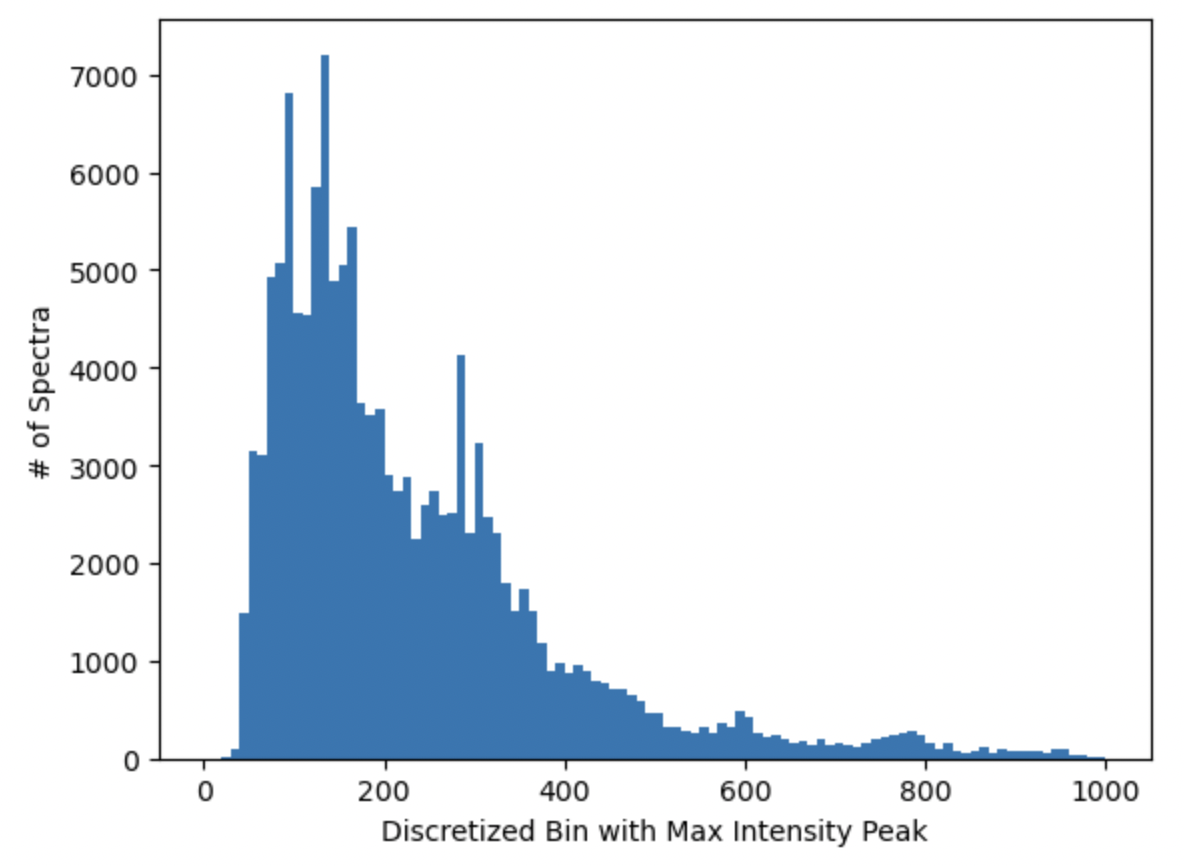
\includegraphics[scale=0.35]{maxbin_hist.png}}
\end{figure}
\subsection{Intended Experimental Results}
Visualized below are toy examples of two graphs we wish to plot for our given models.
\begin{figure}[H]
  \centering
  \centerline{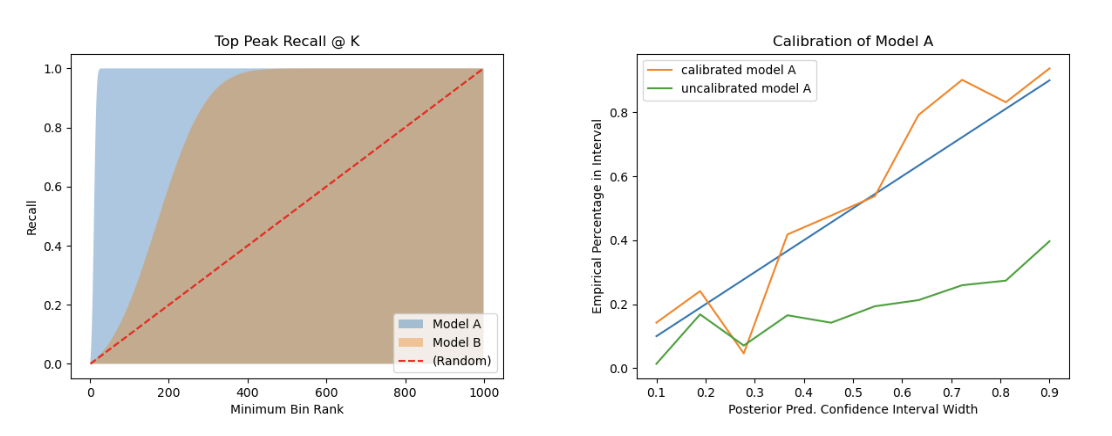
\includegraphics[scale=0.8]{two_plots.png}}
\end{figure}
\textit{Figure 1} (left): The first key plot will be a recall curve for the highest intensity bin across our models. This will involve overlapping three histograms, one for each model, indicating the number of test spectra whose correct highest-peak bin falls within the top $K$ bins.

\textit{Figure 2}: (right): Our second key plot will compare the calibration of our BBB models with different posterior variance assumptions. We calculate calibration as the difference between the expected number of peaks that fall within our confidence intervals according to our model and the actual number of peaks witnessed without our confidence intervals from test-set experimental data. An ideal model shows 1-1 correspond or 'diagonal line' on this plot. 
\subsection{Implementation Plan}
For implementation, we plan to use PyTorch. Each team member has prior experience with it from previous research. We each have past examples of implementing vanilla neural networks in PyTorch, so getting ours up and running should not take too much work. We will have to write PyTorch versions of BBB from scratch. We can use the JAX version of BBB from our homework, however, as a guide. We plan to experiment with Pytorch Lightning to gain some experience in a different styled framework. We plan to experiment with Optuna to gain experience in a hyperparameter optimization framework and help automate parameter selection.

\end{document}
